\documentclass{llncs}
\newcommand{\Section}[1]{\vspace{-8pt}\section{\hskip-1em.~~#1}\vspace{-3pt}}
\newcommand{\SubSection}[1]{\vspace{-3pt}\subsection{\hskip -1em.~~#1}\vspace{-3pt}}
\newcommand{\X}{{\bf X}}
\newcommand{\x}{{\bf x}}
\newcommand{\Y}{{\bf Y}}
\newcommand{\y}{{\bf y}}
\newcommand{\Z}{{\bf Z}}
\newcommand{\z}{{\bf z}}
\newcommand{\bs}{\boldsymbol}
\newcommand{\bSigma}{\boldsymbol \Sigma}
\usepackage{amsmath,amssymb,algorithm,algorithmic}
\usepackage{times}
\usepackage{setspace,verbatim}
\usepackage{epsfig,url}

\newcommand{\argmax}{\operatornamewithlimits{argmax}}
\newcommand{\argmin}{\operatornamewithlimits{argmin}}

\begin{document}
\vspace{-0.1in}
\title{Generating Template Functional Connectivity Networks via Anatomically Constrained Sparse PCA}
\author{Anonymous}
\institute{Anonymous}
\maketitle              
%\vspace{-0.1in}
\begin{abstract}
 Functional connectivity networks have emerged as a powerful tool for studying disease effects on baseline states of neuronal networks in the brain. Traditionally clinicians and medical researchers have been using either totally data driven approaches like Group ICA or exploratory seed region based ROI analysis for constructing functional connectivity networks. Since the Group ICA based approaches do a group decomposition of the time series' images of the entire cohort, it has an averaging effect and erodes away any subject specific characteristics of the network. The ROI based approaches also suffer from the problem of averaging the signal but they are also too conservative as they wrongly assume that the signal lies totally within a predefined region and hence often fail to find any signal. In this paper, we propose a novel approach which integrates ideas from both of these paradigms. Our approach, called Anatomically Constrained Sparse PCA (AC-SPCA) leads to statistically refined definitions of ROIs based on local covariance structure of the time series image. AC-SPCA provides a principled way of incorporating prior information in the form of probabilistic or binary ROIs while still allowing the data to softly modify the original ROI definitions. This allows us to construct subject specific networks with reduced sensitivity to ROI placement. We use our method to graphically describe the default mode network (DMN) connectivity with hippocampus and also use the connectivity patterns to classify MCI vs controls. The results show that properly constructed connectivity networks have more predictive power than hippocampal volume for MCI vs control classification.  Our results also reveal unique relationship between DMN hippocampus network structure and psychometric measurements of memory.

\end{abstract}

\section{Introduction and Related Work}
Over the last  few decades there have been significant breakthroughs in the acquisition of  functional neuroimaging data which has led to an increase in the amount of research efforts directed towards exploration of functional connectivity in the brain. Functional connectivity is defined as the temporal co-activation of neuronal patterns between anatomically separated regions of the brain~\cite{aertsen1989dynamics} and is an indicator of functional communication between these different regions.  Studying the brain as an integrative network of functionally interacting brain regions can shed new light on large scale neuronal communication in the brain and how this communication is impaired in neurodegenerative diseases~\cite{bullmore2009complex,mohammadi2009changes,seeley2009neurodegenerative}. 


Typically, functional connectivity studies measure the level of correlation between the functional time-series of the different brain regions of resting-state blood oxygen level dependent (BOLD) signal~\cite{biswal1997simultaneous,damoiseaux2006consistent,salvador2005neurophysiological}.


There are two predominant approaches for the analysis of functional connectivity, which are described below:
\begin{itemize}
\item {\bf Seed (ROI) Based Approach}:  This is a rather straightforward approach and involves computing the correlation between the time series of a given (preselected) {\it seed} brain region (ROI) against all the other brain regions, resulting in a set of functional connectivity maps of the given brain regions~\cite{biswal1997simultaneous,cordes2000mapping}. These functional connectivity maps can then be used to construct {\it resting-state-networks} of functionally correlated regions in the brain~\cite{damoiseaux2006consistent,fox2005human,beckmann2005investigations}. The {\it seed} region can either be selected based on prior clinical knowledge or it can be selected from the activation map of a separate task dependent fMRI scan.
\item {\bf Learning Based Approaches}: These approaches use statistical techniques to explore functional connectivity in the brain, obviating the need to define a {\it seed} region. Typical methods employed are Principal Component Analysis (PCA)~\cite{friston1998disconnection}, Independent Component Analysis (ICA) or its variants e.g. Group ICA~\cite{beckmann2005investigations,calhoun2001method,petrella2011default} or hierarchical methods~\cite{cordes2002hierarchical,salvador2005neurophysiological}. This class of methods strive to find a set of orthogonal or independent signals in the time series that can explain the resting state activation patterns. ICA based methods are the most popular methods in this setting as they can find a set of independent (uncorrelated) set of signals from whole brain voxel-wise data and also due to the public availability of  tools like (Group ICA of fMRI Toolbox (GIFT)). Subsequently, one can create brain connectivity networks from the outputs of these approaches by computing correlations between the different (independent/orthogonal) signals they find.
 \end{itemize} 


The brain networks found by above approaches are represented as a set of vertices (brain regions) connected by edges which represent the strength of correlation between those two regions~\cite{he2010graph,stam2007graph}. Various independent studies (surveyed here~\cite{van2010exploring}) have consistently found a set of 8 functional connectivity networks in the brain. The networks are shown in Figure 1. One can use a set of key properties of the network graph e.g. clustering coefficient, centrality and modularity to get further insights into the flow of neuronal signals within a network~\cite{he2010graph,stam2007graph}.

The above mentioned approaches for analyzing functional connectivity and constructing brain networks suffer from a variety of problems. Since the Group ICA based approaches do a group decomposition of the time series' images of the entire cohort, it has an averaging effect and erodes away any subject specific characteristics of the network. Moreover, since these approaches are totally data driven, they also lack the clinical interpretability of the results as there is no direct mapping from the regions they highlight and the regions which might be of interest to a clinician. 

The seed (ROI) based approaches also suffer from the problem of averaging the signal. They also wrongly assume that the signal lies totally within a predefined region, however, the important signal may have slightly different boundaries than the scientist's
conception.  The data representation (or spatially varying noise) may
also lead to strong or weak signal within different parts of the seed (ROI).
Such dataset specific information is not taken into account by a
traditional seed (ROI) based approach.  When effects are localized to the selected region, and that region is well-defined, a seed based analysis may
provide the most sensitive testing method.  However, some conditions
involve a network of regions that may not be fully identified.

Due to these shortcomings and due to the fact that decreased/impaired functional connectivity in certain brain networks, for instance, the Default Mode Network (DMN) has association with neurodegenerative disorders e.g. Alzheimer's Disease (AD)~\cite{greicius2004default}, schizophrenia~\cite{liu2008disrupted,whitfield2009hyperactivity}, multiple sclerosis (MS)~\cite{lowe2008resting}, mild cognitive impairment (MCI)~\cite{petrella2011default}, it has become even more imperative to come up with improved statistical analysis methods which can efficiently leverage the scarce patient BOLD fMRI data that is typically available. 

In this paper, we propose a method that integrates ideas from both the seed (ROI) based and learning based approaches. Our contributions in this paper are three fold.

\begin{enumerate}
\item Our main approach, Anatomically Constrained Sparse PCA (AC-SPCA), which in addition to being data driven, incorporates prior knowledge in terms of seed ROIs, to construct a subject specific functional network.
\item A novel conjugate gradient based efficient method for optimization of the AC-SPCA objective. 
\item Publicly available implementation of our approach in C++.
\end{enumerate}

AC-SPCA allows an initial binary or probabilistic ROI to adapt to
the underlying covariation within the data and thus has advantages of
SPCA.  At the same time, AC-SPCA maintains proximity to (and the
locality of) the original region and thus has advantages of the
standard seed (ROI) approach.  AC-SPCA also maintains positivity in the
estimated anatomically-constrained eigenvector, thereby keeping seed (ROI)
interpretability. This allows us to modify the definitions of labels to capture the variation in dataset (a given subject's time series) while still staying close to the initial seed (ROI) definitions. AC-SPCA therefore produces
labelings with ``soft'' weighted averages and as we show in the
experimental section, are more sensitive to the underlying
brain data than a standard seed (ROI). One can define a set of seed ROIs using, for instance, Automated Anatomical Labels (AAL)~\cite{tzourio2002automated}.

Our approach provides a principled way of incorporating priors in a totally data driven approach based on PCA. Our optimization objective provides a tradeoff between 1). staying close to the initial ROI definitions and 2). allowing data to lead the exploratory analysis by explaining variance through PCA. A good way to think about this is as ROI definitions forcing us to be {\em conservative} and staying close to the initial definitions e.g. AAL labels; on the other hand the SPCA component gives us {\em liberty} to be more exploratory and just trust the given data. The tradeoff between the two competing paradigms is defined by user tunable (prior strength) parameter, which is chosen via cross validation on a separately held validation set. 

AC-SPCA does a prior constrained sparse decomposition of each subject's time series image separately, so it doesn't suffer from the problem of averaging as Group ICA does. Moreover, the priors help us maintain a direct correspondence between the anatomy of the same regions across different subjects hence leading to better clinical interpretability.

The remaining paper is organized as follows; in next section we provide the details of AC-SPCA and provide an algorithm which implements our approach. In Section 3, we provide experimental results in which we use our approach to graphically describe the default mode network (DMN) connectivity with hippocampus. We also use the connectivity patterns to classify MCI vs controls and also study the relationship between DMN hippocampus network structure and psychometric measurements of memory. We conclude with a brief summary in Section 4.


 %This has lead to a substantial interest in using sophisticated statistical methods to analyze and explore this data. Methods like Principal Component Analysis (PCA), Independent Component Analysis (ICA), Canonical Correlation Analysis (CCA) and their robust and sparse variants~\cite{Witten2009b,Avants2010b} have been the workhorse of brain and neuro imaging fields as they provide key insights into the data in a totally data driven way. 

%Particularly they find directions of maximum variance in data or its close variant and show the signal to lie in a small number of succinct regions in brain. 




\section{ Anatomically Constrained Sparse Principal Component Analysis: AC-SPCA}
The class of methods encompassing sparse principal components analysis (SPCA)~\cite{zou2006sparse,Witten2009b,d2007direct} and singular value decomposition~\cite{sill2011robust} form the basis for the approach proposed here. 


More formally, lets define a set of $n$, $t\times p$ (rows by columns) matrices $\{\bf X_m\}_{m=1}^n$ where $t$ is the number of total time points, $p$ is the number of total voxels and each ${\bf X}_m$ matrix derives from an observed subject's BOLD fMRI image.
 Also, lets assume that we have a prior matrix {$\bf M$} whose each row corresponds to a separate prior (total {\bf k} of them) and each column (total {\bf p} of them) contains the probability of a particular voxel belonging to that prior. 


We are interested in sparse decomposition of the ${\bf X}_m$ matrices constrained by the anatomical priors {\bf M} which should give us a $t \times k$ matrix for each subject where each of the $k$ eigenvectors explains the variance in the corresponding anatomical region specified by the prior.


A standard data driven approach PCA would ignore the prior matrix {\bf M} completely and just try to find combinations of voxels that explain the most variance. The objective it optimizes is:

\begin{equation}
{\bf v_i^*}= \argmax_{{\bf v_i},{\bf \|v_i\|}=1} {\bf v_i}^{\top}{\bf X^{\top}X}{\bf v_i}
\label{pca}
\end{equation}
where {$\bf v_i^*$} is the $i^{th}$ direction of maximum variance (called eigenvector) of data matrix {\bf X}. These vectors when plotted on the image highlight regions which are
relevant for explaining variance in the data. Since, we have ${\bf p \gg n}$, the above is an ill-posed problem and we need sparsity in eigenvectors, which gives rise to Sparse PCA. The objective is exactly the same as Equation~\ref{pca} except that now we have an additional sparsity penalty ($\|\bf v _i\|_0$) on eigenvectors.  Exact optimization of Sparse PCA is an NP-hard problem and usually its solved by relaxing the sparseness condition~\cite{zou2006sparse,Witten2009b}.




Our proposed algorithm AC-SPCA builds on Equation~\ref{pca} and adds an additional term to the objective for incorporating prior information. Basically, it says that instead of finding the eigenvectors of the data covariance matrix (as a totally data driven approach would do), find the eigenvectors of the transformed data covariance matrix obtained by ``regularizing'' it by the prior information. An important consequence of this is that we are not confining our data driven priors to lie in the original seed ROIs rather we are encouraging them to find ways to explain data variance but in this new ``prior regularized'' space. The modified objective is given below:
\begin{eqnarray}
\label{ppca}
{\bf v_i^*}&=& \argmax_{{\bf v_i},{\bf \|v_i\|}=1} {\bf v_i}^{\top}\left((1-\lambda)\cdot{\bf X^{\top}X +  \lambda\cdot M^s_i\otimes M^s_i}\right){\bf w_i}  \\
\nonumber
&&such\;that\;\|{\bf v_i}\|_0=\gamma
\end{eqnarray}
where ${\bf M^s_i}$ is  the ``smoothed'' prior corresponding to the $i^{th}$ eigenvector and is itself a vector of size (${\bf 1\times p}$). $\otimes$ is the outer product operator and is defined as $\bf MM^{\top}$.  $\lambda$ is a user tunable parameter which controls the tradeoff between the influence of data and prior and should be typically tuned on a held out validation set in the absence of other knowledge. 

Its easy to see that smaller values of $\lambda$ suggest that we trust prior more and as $\lambda$ is increased we want our eigenvectors {\bf v} to be influenced more and more by the data. Sparseness is enforced by a soft-thresholding algorithm as in~\cite{zou2006sparse,Witten2009b}. We denote this function as $S(v,\gamma)$ and (in an adhoc manner) allow it to also reject isolated voxels (i.e. we provide a cluster threshold as in VBM). In our experiments, we typically set $\gamma$ to ensure that only $\sim5\%$ of the voxels have non zero weight.


 It is important to note that the matrix ${(1-\lambda)\cdot \bf X^{\top}X +  \lambda\cdot M^s_i\otimes M^s_i}$ is no longer symmetric, so after eigen decomposition, its left and right eigenvectors won't be the same. We are however interested in finding the left eigenvectors. 

%Also, it is important to note that we set the sparsity parameter $\eta$ automatically as $\frac{Number\;\;of\;\;voxels\;\;in\;\;Prior\;\;ROI}{Total\;\;Number\;\;of\;\;Voxels\;\;in\;\;Brain}$. 

%Figure~\ref{fig:priorvary} uses example face data to show the effect of varying the $\lambda$  parameter on the AC-PCA performance. As mentioned earlier, we choose $\lambda$ by cross-validation on a validation set.

\subsection{An Algorithm for AC-SPCA}
The algorithm for AC-SPCA presented below in Algorithms~\ref{algo1},~\ref{algo2}. In our initialization, we find a matrix {\bf U} which minimizes the reconstruction error  $\bf \|X - UV^{\top}\|^2$, where {\bf U} is $n\times k$ matrix and {\bf V} is a {$p \times k$} matrix. In our case {\bf V}, the set of eigenvectors are initialized by the prior matrix. We then factor (``partial'') out the effect of all other priors except the prior under consideration. Next we optimize the eigenvectors using Sparse Partial Conjugate Gradient (SPCG) algorithm, which is an iterative procedure and works by projecting the eigenvectors to the sparse solution space repeatedly, till convergence (based on rayleigh coefficient). It is important to note that in the SPCG algorithm, we use two engineering tricks which prevent us from explicitly computing the big $p\times p$ matrix.  First of all, for the multiplication $\bf X^{\top}Xv_i$, we first compute $\bf Xv_i$ and then multiply it with $\bf X^{\top}$, rather than multiplying $\bf X^{\top}X$ first. Secondly, when computing $({\bf M^s\otimes M^s}){\bf v_i}$, we first compute the inner product of ${\bf M^s_i}$ and $\bf v_i$, and then compute a second inner product of the result with  $\bf v_i$; its easy to verify that we get the answer as by directly computing $({\bf M^s\otimes M^s}){\bf v_i}$.

\begin{algorithm}[htdp]
\small \caption{\bf Anatomically Constrained Sparse Principal Component Analysis: AC-SPCA}
\label{algo1}
\begin{algorithmic}[1]
\STATE Input:  \{{\bf X}, {$\bf M^s$}, $\lambda$, $\gamma$ \} .
\STATE Normalize the data matrix {\bf X} by  mean centering it.
\FOR {i=1 to k}
\STATE Initialize the $i^{th}$ eigenvector $\bf v_{i} \gets M^s_i$ based on the corresponding prior.
\STATE Compute {$\bf u_i$} i.e. the $i^{th}$ row of the $\bf U$ matrix by minimizing the reconstruction error as ${\bf u_i^*}= \argmin_{u_i} \|{\bf x_i} - {\bf u_i}\otimes {\bf v_i} \|_2^2$.
\ENDFOR
\FOR {i=1 to k}
\STATE Compute the partial {\bf X} matrix as: ${\bf X}_{\backslash i}= {\bf X}- \sum_{j=1, j\neq i}^{k}  {\bf u_j}\otimes {\bf v_j}$
\STATE  ${\bf v_i}$ $\gets$ {\bf SPCG}$({\bf X}_{\backslash i},\lambda,\gamma, {\bf v_i})$ //Perform Sparse Partial Conjugate Gradient.
\STATE Normalize the eigenvector ${\bf v_i}$ $\gets$ ${\bf v_i}/\|{\bf v_i}\|$
\STATE ${\bf v_i}$ $\gets$  $S(v,\gamma)$ //Soft-Max and Cluster Thresholding.
\ENDFOR
%\STATE j $\leftarrow$ j+1
%\ENDWHILE
\STATE Output:  $\{{\bf v}\}_{i=1}^{k}$
\end{algorithmic}
\end{algorithm}



\begin{algorithm}[htdp]
\small \caption{\bf Sparse Partial Conjugate Gradient: SPCG}
\label{algo2}
\begin{algorithmic}[1]
\STATE Input:  \{${\bf X}_{\backslash i},\lambda,\gamma, {\bf v_i}$ \} .
\STATE Compute Rayleigh Coefficient $R^0$=$\frac{{\bf v}^{\top}{\bf X}_{\backslash i}{\bf v}}{{\bf v}^{\top}{\bf v}}$
\STATE ${\bf e_i}$ $\gets$ ${\bf X}{\bf v_i}$ 
\STATE ${\bf gX}_i$ $\gets$ $(1-\lambda)\cdot{\bf X^{\top}e_i}$  //Gradient of the data term in the objective.
\STATE $f_i  \gets  <{\bf M^s_i, \bf v_i}>$ // $<,>$ indicates inner product.
\STATE ${\bf gP}_i$ $\gets$ $\lambda\cdot <f_i,{\bf v_i}>$   //Gradient of the prior term in the objective.
\STATE $j \gets 0$ //Iteration Counter.
\STATE ${\bf p_i^j} \gets \lambda\cdot e_i + (1-\lambda)$ +{\bf gP}
\STATE ${\bf v_i^j} \gets {\bf v_i}$
\STATE ${\bf l_i^j} \gets {\bf v_i^j}$
\WHILE {$R^j <R^{j-1}$}
\STATE ${\bf n_i^{j}}$ $\gets$ $(1-\lambda)\cdot {\bf gX} + {\bf gP}$
\STATE $\eta \gets  \|{\bf n_i^{j}}{\bf n_i^{j}}\|_2^2 / \|{\bf l_i^j}{\bf l_i^j}\|_2^2$
\STATE ${\bf l_i^j} \gets {\bf n_i^j}$
\STATE ${\bf v_i^{j}}$ $\gets$ $ {\bf v_i^{j}} + \eta\cdot {\bf n_i^{j}}$
\STATE  ${\bf v_i^j}$ $\gets$ ${\bf v_i^j}/\|{\bf v_i^j}\|$
\STATE ${\bf p_i^j} \gets \lambda\cdot e_i + (1-\lambda)$ +{\bf gP}
\STATE Compute $R^j \gets <p_i^j,p_i^j>/<v_i^j,v_i^j>$ 
\STATE $j \gets j+1$
\ENDWHILE
\STATE Output:  $\{{\bf v}\}_{i=1}^{k}$
\end{algorithmic}
\end{algorithm}

%\STATE Soft-Max Sparseness:  ${\bf v_i^{j}}  \leftarrow (\|{\bf v_i^{j}}\|  - max({\bf v_i^{j}})*\eta)_+ Sign({\bf v_i^{j}})$ //Note that $\eta$ is set automatically as described earlier.




\iffalse
\begin{figure*}
\begin{center}
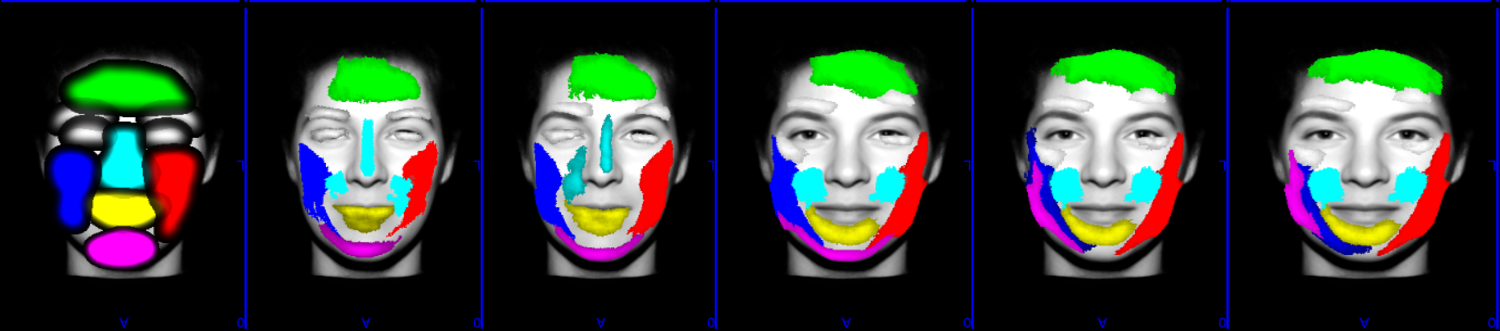
\includegraphics[width=\linewidth]{fig2.pdf} 
\end{center}
\vspace{-0.2in}
\caption{(AC-PCA) outputs for $\lambda=[0.0,0.2,0.5,2.0,5.0,10.0]$ from left to right. Note that $\lambda =0$ corresponds to using only prior ROIs and as $\lambda$ is increased effect of data increases. This is evident from the fact that with increasing $\lambda$ our priors especially around {\em nose, eyes and eyebrows} are getting washed away.}
\label{fig:priorvary}
\end{figure*}







\section{Experimental Results}
In this section we show the performance of our approach on cortical thickness images. Our data consists of images from 222 individuals with equal number of males and females of whom 122 were diagnosed clinically with Mild Cognitive Impairment (MCI) and the remaining 100 were normal controls. The average age of the cohort was 71.33. %add info. about age and gender
All images were acquired with a Siemens Trio 3.0 Tesla MRI scanner. The analysis of T1 images was done using publicly available Advanced Normalization Tools (ANTS, \url{http://www.picsl.upenn.edu/ANTS/}) and the associated pipelining framework PipeDream ({\url{http://sourceforge.net/projects/neuropipedream/}) which mapped each subject to an existing, elderly/neurodegenerative population template, built from images acquired from the same scanner and imaging parameters.

We used two cortical label (probabilistic ROIs) definitions for our experiments 1). Non-Rigid Image Registration Evaluation Project (NIREP),  (\url{http://www.nirep.org/}), 32 labels in total and  2). LONI Probabilistic Brain Atlas (LPBA40)~\cite{lpba}, 55 labels in total.


We ran AC-PCA independently for each label set with varying values of prior strengths, $\lambda =[0.1,0.2,0.5,1.0,2.0,5.0,10.0,20.0]$.


\begin{figure*}
\begin{center}
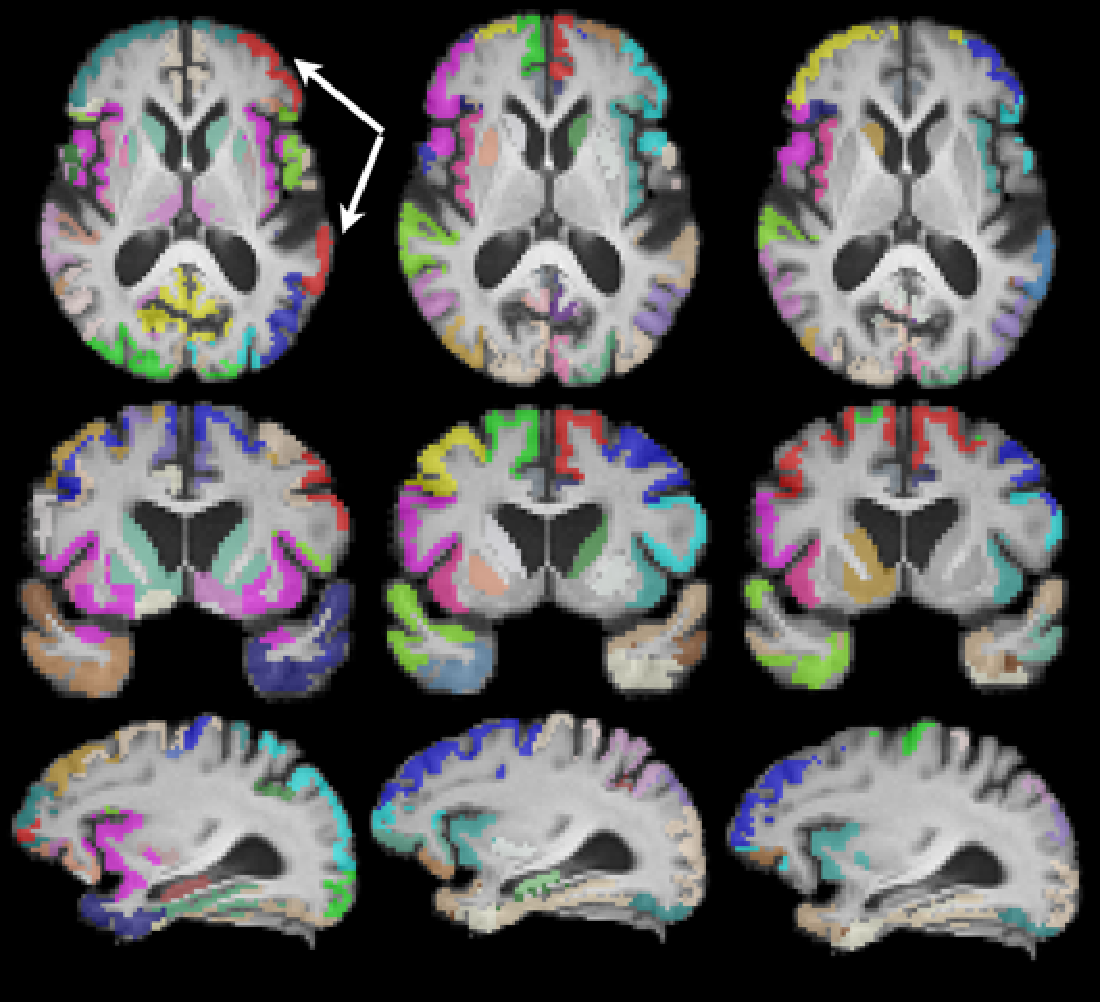
\includegraphics[width=0.7\linewidth]{lpba.pdf} 
\end{center}
\vspace{-0.2in}
\caption{Results for LPBA40 labels. Left to right- Unconstrained PCA, prior LPBA labels, AC-PCA labels. The arrows show left frontal gyrus and the left superior temporal gyrus. The value of the prior strength $\lambda$ for AC-PCA is $0.2$, chosen on validation set. Note that not all the 55 anatomical priors can be seen in this slice.}
\label{fig:priorlpba}
\end{figure*}


\subsection{Qualitative Results}

The figures below show slices of axial and sagittal section labelings for unconstrained PCA, true cortical labels (NIREP and LPBA40) and prior constrained PCA (AC-PCA).

% As can be seen from the figures, the prior constrained labelings have been modified from their prior anatomical definitions (i.e. NIREP or LPBA) based on evidence from data. However, unlike unconstrained PCA, the AC-PCA labels are more spatially constrained and do not generate the same label for distant but correlated brain structures. 
%As can be seen from the figures, there is a one-one correspondence between prior anatomical labels and the labeling generated by AC-PCA as we have constrained them to stay near to their prior labels, however such a correspondence does not exist between the labels generated by unconstrained PCA and prior labels  

Note that in the unconstrained PCA, the same label is assigned to parts of the left frontal gyrus and the left superior temporal gyrus (shown by arrows in figure) since it has no notion of anatomy; on the other hand, AC-PCA, since it is anatomical prior driven does not join distant structures which aids interpretability.

Another interesting observation is that both AC-PCA and unconstrained PCA have assigned  the same label to corresponding regions in the left and right hemispheres. This occurs less frequently in AC-PCA as we have constrained it via anatomical priors.  %The anatomical constraint is less effective for structures close to the mid-line of the brain because these structures are closer to the corresponding structure on the other hemisphere.
%%since based on euclidean distance structures on opposite hemispheres which are close to each other can have same label.


\begin{figure*}
\begin{center}
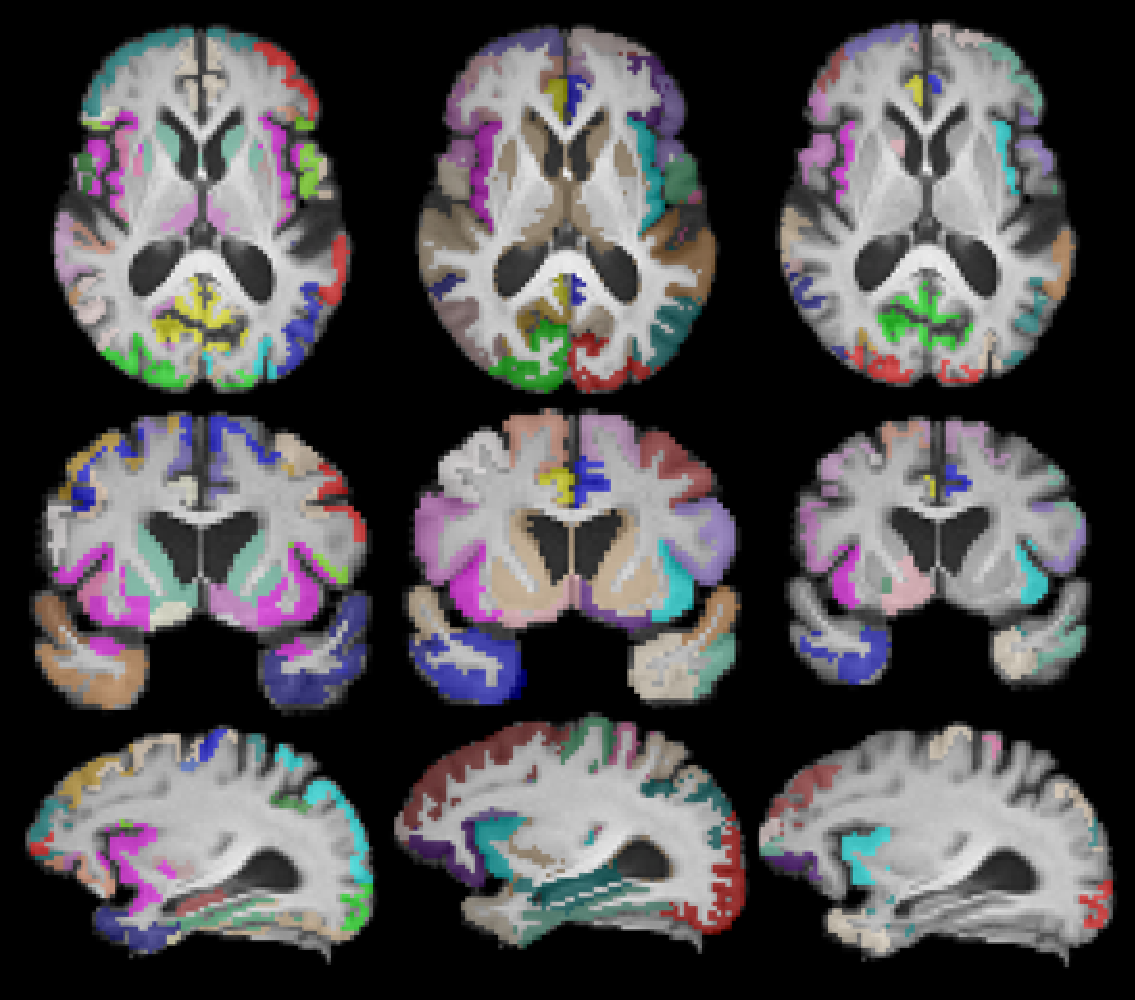
\includegraphics[width=0.7\linewidth]{nirep.pdf} 
\end{center}
\vspace{-0.2in}
\caption{Results for NIREP labels. Left to right- Unconstrained PCA, prior NIREP labels, AC-PCA labels. The value of the prior strength $\lambda$ for AC-PCA is $0.5$, chosen on validation set. Note that not all the 32 anatomical priors can be seen in this slice.}
\label{fig:priornirep}
\end{figure*}


\subsection{Classification of MCI vs Controls}

We hypothesize that AC-PCA will improve over basic ROIs on (MCI vs Controls) classification results by allowing the summary
measurements derived from the imaging data to adapt to the underlying signal.  We also hypothesize that AC-PCA locality will improve over
unconstrained PCA-based classification.

We use the projections (eigenvectors projected onto the data matrix) resulting from unconstrained PCA, AC-PCA and prior cortical labels to distinguish individuals with Mild Cognitive Impairment (MCI) from normal aging individuals~\cite{Zhou2011,Chen2010}. 
Since it is a classification problem, we used logistic regression and randomly split the data into training ($80\%$), validation ($10\%$) and testing ($10\%$). Firstly, we use cross validation to determine the best value of prior strength parameter ($\lambda$); we train on the training data and test on validation data with varying prior strengths as mentioned above and then choose the best value of prior strength as the one which gave the least classification error on the validation set.  The best prior strength value was $\lambda =0.5$ for NIREP labels and $\lambda=0.2$ for LPBA40 labels. 

Next, with these values of $\lambda$ we trained AC-PCA on the entire training and validation set and tested on the test set. This whole procedure was repeated 10000 times and the classification accuracies are given in Table 1.

As can be seen from the table, the AC-PCA significantly (paired t-test) outperforms unconstrained PCA as well as the approach which just uses cortical ROI labels hence leading to a classifier which can better distinguish MCI patients from normal controls. 


\begin{table}
\begin{center}
\begin{small}
\begin{tabular}{|c|c|c|c|}
\hline
 Label Set& Unconstrained PCA ($\mu\pm\sigma$) & ROI Cortical Labels ($\mu\pm\sigma$) & AC-PCA ($\mu\pm\sigma$)  \\
\hline
 NIREP& $62.58\% \pm 4.5\%$&$66.05\pm 3.9\%$ &${\bf 67.96\%\pm 2.3\%}$\\
 LPBA40&$62.58\% \pm 4.5\%$&$65.95\%\pm3.6\%$ &${\bf 67.15\%\pm 3.2\%}$\\ 
   \hline
\end{tabular}
\end{small}
\vspace{0.1in}
\caption{Test Set classification accuracies averaged over 10000 runs (More details in text). AC-PCA is significantly ($p-val <0.0001$ in paired t-test) better than Unconstrained PCA and ROI Cortical Labels}
\end{center}
\end{table}


\section{Conclusion}
In this paper we proposed a novel approach for incorporating prior information in the form of anatomical priors into totally data driven approaches like PCA. We augmented the basic PCA objective to take into account prior anatomical information and proposed a fast modified Arnoldi iteration algorithm to solve the optimization problem. 
We also illustrated the benefits of our approach over standard unconstrained PCA as well as ROI based analysis by experiments on cortical thickness images which shows the superiority of AC-PCA for MCI classification compared to ROI and unconstrained PCA (a totally data based approach).  Besides this, the labels output by AC-PCA readily lend themselves
to interpretability by clinicians and other medical researchers as there is a one-one correspondence between the AC-PCA labels and prior anatomical labels, unlike totally data driven approaches like unconstrained PCA.
\fi

%\vspace{-0.2in}
\bibliographystyle{IEEEbib}
\bibliography{./ipmi}

\end{document}

